\documentclass{sigchi}

% Use this section to set the ACM copyright statement (e.g. for
% preprints).  Consult the conference website for the camera-ready
% copyright statement.

% Copyright
\CopyrightYear{2020}
%\setcopyright{acmcopyright}
\setcopyright{acmlicensed}
%\setcopyright{rightsretained}
%\setcopyright{usgov}
%\setcopyright{usgovmixed}
%\setcopyright{cagov}
%\setcopyright{cagovmixed}
% DOI
\doi{https://doi.org/10.1145/3313831.XXXXXXX}
% ISBN
\isbn{978-1-4503-6708-0/20/04}
%Conference
\conferenceinfo{CHI'20,}{April  25--30, 2020, Honolulu, HI, USA}
%Price
\acmPrice{\$15.00}

% Use this command to override the default ACM copyright statement
% (e.g. for preprints).  Consult the conference website for the
% camera-ready copyright statement.

%% HOW TO OVERRIDE THE DEFAULT COPYRIGHT STRIP --
%% Please note you need to make sure the copy for your specific
%% license is used here!
% \toappear{
% Permission to make digital or hard copies of all or part of this work
% for personal or classroom use is granted without fee provided that
% copies are not made or distributed for profit or commercial advantage
% and that copies bear this notice and the full citation on the first
% page. Copyrights for components of this work owned by others than ACM
% must be honored. Abstracting with credit is permitted. To copy
% otherwise, or republish, to post on servers or to redistribute to
% lists, requires prior specific permission and/or a fee. Request
% permissions from \href{mailto:Permissions@acm.org}{Permissions@acm.org}. \\
% \emph{CHI '16},  May 07--12, 2016, San Jose, CA, USA \\
% ACM xxx-x-xxxx-xxxx-x/xx/xx\ldots \$15.00 \\
% DOI: \url{http://dx.doi.org/xx.xxxx/xxxxxxx.xxxxxxx}
% }

% Arabic page numbers for submission.  Remove this line to eliminate
% page numbers for the camera ready copy
% \pagenumbering{arabic}

% Load basic packages
\usepackage{balance}       % to better equalize the last page
\usepackage{graphics}      % for EPS, load graphicx instead 
\usepackage[T1]{fontenc}   % for umlauts and other diaeresis
\usepackage{txfonts}
\usepackage{mathptmx}
\usepackage[pdflang={en-US},pdftex]{hyperref}
\usepackage{color}
\usepackage{booktabs}
\usepackage{textcomp}
\usepackage{graphicx}

% Some optional stuff you might like/need.
\usepackage{microtype}        % Improved Tracking and Kerning
% \usepackage[all]{hypcap}    % Fixes bug in hyperref caption linking
\usepackage{ccicons}          % Cite your images correctly!
% \usepackage[utf8]{inputenc} % for a UTF8 editor only

% If you want to use todo notes, marginpars etc. during creation of
% your draft document, you have to enable the "chi_draft" option for
% the document class. To do this, change the very first line to:
% "\documentclass[chi_draft]{sigchi}". You can then place todo notes
% by using the "\todo{...}"  command. Make sure to disable the draft
% option again before submitting your final document.
\usepackage{todonotes}

% Paper metadata (use plain text, for PDF inclusion and later
% re-using, if desired).  Use \emtpyauthor when submitting for review
% so you remain anonymous.
\def\plaintitle{CSCM69: Human-Centred Perspectives and Methods\\Coursework 1}
\def\plainauthor{Andy Gray}
\def\emptyauthor{}
\def\plainkeywords{Authors' choice; of terms; separated; by
  semicolons; include commas, within terms only; this section is required.}
\def\plaingeneralterms{Documentation, Standardization}

% llt: Define a global style for URLs, rather that the default one
\makeatletter
\def\url@leostyle{%
  \@ifundefined{selectfont}{
    \def\UrlFont{\sf}
  }{
    \def\UrlFont{\small\bf\ttfamily}
  }}
\makeatother
\urlstyle{leo}

% To make various LaTeX processors do the right thing with page size.
\def\pprw{8.5in}
\def\pprh{11in}
\special{papersize=\pprw,\pprh}
\setlength{\paperwidth}{\pprw}
\setlength{\paperheight}{\pprh}
\setlength{\pdfpagewidth}{\pprw}
\setlength{\pdfpageheight}{\pprh}

% Make sure hyperref comes last of your loaded packages, to give it a
% fighting chance of not being over-written, since its job is to
% redefine many LaTeX commands.
\definecolor{linkColor}{RGB}{6,125,233}
\hypersetup{%
  pdftitle={\plaintitle},
% Use \plainauthor for final version.
%  pdfauthor={\plainauthor},
  pdfauthor={\emptyauthor},
  pdfkeywords={\plainkeywords},
  pdfdisplaydoctitle=true, % For Accessibility
  bookmarksnumbered,
  pdfstartview={FitH},
  colorlinks,
  citecolor=black,
  filecolor=black,
  linkcolor=black,
  urlcolor=linkColor,
  breaklinks=true,
  hypertexnames=false}

% create a shortcut to typeset table headings
% \newcommand\tabhead[1]{\small\textbf{#1}}

% End of preamble. Here it comes the document.
\begin{document}

\title{\plaintitle}

\numberofauthors{1}
\author{%
  \alignauthor{Andy Gray\\
    \affaddr{445348}\\
    \affaddr{Swansea, Wales}\\
    \email{445348@swansea.ac.uk}}
}
\maketitle

\begin{abstract}
	With 58\% of the world on the internet \cite{126_sm_facts}, people are becoming more and more connected to the digital world. While this digital world brings a lot of newfound access and freedom to many. Allowing people to connect with other people that do not live in the same country or people they have never met before in person. While the internet has brought about some fantastic achievements, it has, for some, brought a lot of side effects. At the cost of their mental health. We look at how the more significant the time spend on social media can affect, especially in women, their self-esteem and mental health. While also critiquing Instagram's creator's page overview and providing ideas that will take focus away from the creator's metrics, and focus on the individual instead.
  
\end{abstract}


% ACM Classfication

\begin{CCSXML}
<ccs2012>
<concept>
<concept_id>10003120.10003121</concept_id>
<concept_desc>Human-centered computing~Human computer interaction (HCI)</concept_desc>
<concept_significance>500</concept_significance>
</concept>
<concept>
<concept_id>10003120.10003121.10003125.10011752</concept_id>
<concept_desc>Human-centered computing~Haptic devices</concept_desc>
<concept_significance>300</concept_significance>
</concept>
<concept>
<concept_id>10003120.10003121.10003122.10003334</concept_id>
<concept_desc>Human-centered computing~User studies</concept_desc>
<concept_significance>100</concept_significance>
</concept>
</ccs2012>
\end{CCSXML}

\ccsdesc[500]{Human-centered computing~Human computer interaction (HCI)}
\ccsdesc[300]{Human-centered computing~Haptic devices}
\ccsdesc[100]{Human-centered computing~User studies}

% Author Keywords
\keywords{\plainkeywords}

% Print the classficiation codes
\printccsdesc
Please use the 2012 Classifiers and see this link to embed them in the text: \url{https://dl.acm.org/ccs/ccs_flat.cfm}



\section{Introduction}
	As of December 2019, the internet has 4.54 billion users, while the world has 7.8 billion people \cite{126_sm_facts}. As these figures show, there is a lot of users on the internet. These figures show that 58\% of the world's population is online, which is a lot of people. Out of these 4.54 billion internet users, 3.725 billion users are active on social media to an average of 142 minutes a day \cite{126_sm_facts}. Facebook accounts for about 21\% of all of the social media referral traffic in the world. It is also driving 23\% of all traffic across all of the internet \cite{47_sm_facts, 126_sm_facts}. However, there are many other social media outlets available. Some of these include Instagram, Pinterest, LinkedIn, YouTube, Twitter, TikTok and Snap Chat, to name a few.
	
	Another exam of how social media has become ingrained into our everyday lives is that approximately 80\% of world leaders have Twitter accounts \cite{47_sm_facts}. However, the frequency of the tweets will vary depending on one leader to another. Between October 2018 and 2019, social media users grew by 328 million, which works out at ten new social media users per second \cite{126_sm_facts}.
	
	While social media can bring up many conversations, some of these conversations include privacy, as only 25\% of Facebook users bother to check or adjust their privacy settings \cite{47_sm_facts}. Other discussions include social medias ethics about them needing to holding so much information about you, which has recently got brought to light with the Cambridge Analytica fiasco. Mental and substance use disorders are the leading cause of years lived with disability worldwide and in 2010 accounted for 7.4\% of years of productive life lost due to disability \cite{gkotsis2017characterisation}. We feel more needs to be asked of what the social media giants are doing to tackle mental health problems, as almost one-quarter of Facebook users check the site five times or more per day \cite{47_sm_facts}. Also, the median number of friends the average Millennial Facebook user has in their network is 250. However, are these people that they know or just random connections. While being a teacher previous, are a crucial topic concerning safeguarding and the peoples' lives and is it disconnecting them from the real world more and more?
	
	We will look to first look into what the literature says about social media and its effects on mental health. We will then look to critique a tool. The tool that we will be critiquing is the creator's overview section on their profile on Instagram. We will then be looking at an innovation, based around the Instagram tool, that we think will help with some of the issues raised in the literature review.


\section{Synthesising the Papers}
	Young people are frequently turning to sites such as Facebook and Twitter to escape from the outside pressures threatening their mental health \cite{boyd2014s}. Adolescents living in many countries (including low, middle and high income) have seen information and communication technologies such as social media become integral to their education, culture and social life \cite{allen2014social, van2013culture}. Evidence suggests social media use is associated with mental health in young people, but underlying processes are not well understood. However, it got found that the extent of the association between social media use and depressive symptoms was larger for girls than for boys. Compared with 1–3 h of daily use: 3 to < 5 h 26\% increase in scores vs 21\%; $\geq$ 5h 50\% compared to 35\% for girls and boys respectively \cite{kelly2018social}. Another study also showed that although there is some indication of a general connection between adolescent social media use and negative indicators of health, for example, sleep problems, anxiety, lower self-esteem \cite{underwood2017power, scott2018fear}. However, as most research on the link between social media activity and psychosocial adjustment gets based on young adults. It, therefore, is not clear how well the findings apply to the generation of adolescents who never known a world without such platforms and who presumably have frequent contact with social media \cite{barry2017adolescent}. However, despite the relative significance of protecting mental health and emotional wellbeing, adolescents tend to have limited knowledge of what it means to be mentally healthy or how to maintain this status \cite{dogra2012nigerian}.
	
	%% Not finished here down
	Although social media may be facilitating new forms of communication and social connection \cite{baker2008blogging}, initially there were worries about the amount of time young people were spending online. This concern was due to internet use was being linked to a decrease in face-to-face contact, increased social isolation, stress, depression and sleep deprivation \cite{kraut1998internet, espinoza2011pervasiveness}. It gets claimed to facilitate offensive and harmful behaviour, arguably detrimental to mental health \cite{mesch2009parental}. However, some research contradicts this 'internet paradox' \cite{o2018social} by presenting evidence that such negative traits disappear once internet novices became more mature users of ICT \cite{kraut2002internet}. Furthermore, the effects of internet usage upon those with conditions such as depression got argued to be dependent upon the purpose of its use and the pre-existing social resources of individual users \cite{bessiere2008effects}. Nevertheless, policymakers have proceeded to express anxieties concerning the level of risk that adolescents get exposed to on social media \cite{boyd2014s}.
	
	Most important finding was that social media activity, for example, the number of accounts adolescents have and their self-reported frequesncy of checking social media, was moderately, positively related to the Fear of Missing Out (FoMO) and loneliness. Additionally, as well as with parent-reported hyperactivity or impulsivity, anxiety, and depression \cite{barry2017adolescent}. The latter findings are particularly unique in that they cannot get explained by shared source varience. These unexplained findings were due to adolescent-reported social media activity was associated with externalising and internalising symptoms that were reported by parents. However, a teen otherwise engaged in mundane activities. These activities include waiting in line, doing homework, being out with friends. Hyperactivity or impulsivity teens may have a more incredible urge to engage with social media. That is if the opportunity were to exist \cite{barry2017adolescent}. The youth with higher internalising symptoms may get drawn to social media as a means to connect to others. Admittedly, adolescent-reported loneliness got related to having a higher number of social media accounts in this sample. Previous evidence suggests that adolescent females with internalising traits may use social media in a way consistent with co-rumination with peers who have similar experiences or who offer support \cite{ehrenreich2016adolescents}.
	
	Additionally, an adolescent's perception that he or she does not compare well to others as seen on social media or does not have the kinds of affiliations with others that he or she perceives on social media may increase internalising traits. Thus, a perceived discrepancy between one's own experiences and the positive experiences of others that one is missing out on maybe a concequence of social media activity. At face value, these findings are suggestive of negative mental heath correlates of having a higher number of social media accounts, yet as has been demonstrated with depression \cite{frison2016short}, it cannot be determined if these mental health indices are indeed an outcome or precursor of teen involvement with social media and social media experiences such as peer victimisation \cite{barry2017adolescent}.

	More significant amounts of social media usage time do get associated with more online harassment, poor sleep, low self-esteem and poor body image. In turn, these related to a higher level of depressive symptom scores \cite{kelly2018social}. Multiple potential pathways were apparent to reach this outcome. An example pathway is the more significant amount of hours spent on social media related to the amount of body weight dissatisfaction. A user with $\geq$ 5h resulted in 31\% more likely to be dissatisfied, which in turn linked to depressive symptom scores directly and indirectly via self-esteem, including body dissatisfaction being 15\% higher in depressive symptom scores \cite{kelly2018social}.

\section{Critiquing a Tool}

%	\begin{figure}
%		\begin{center}
%			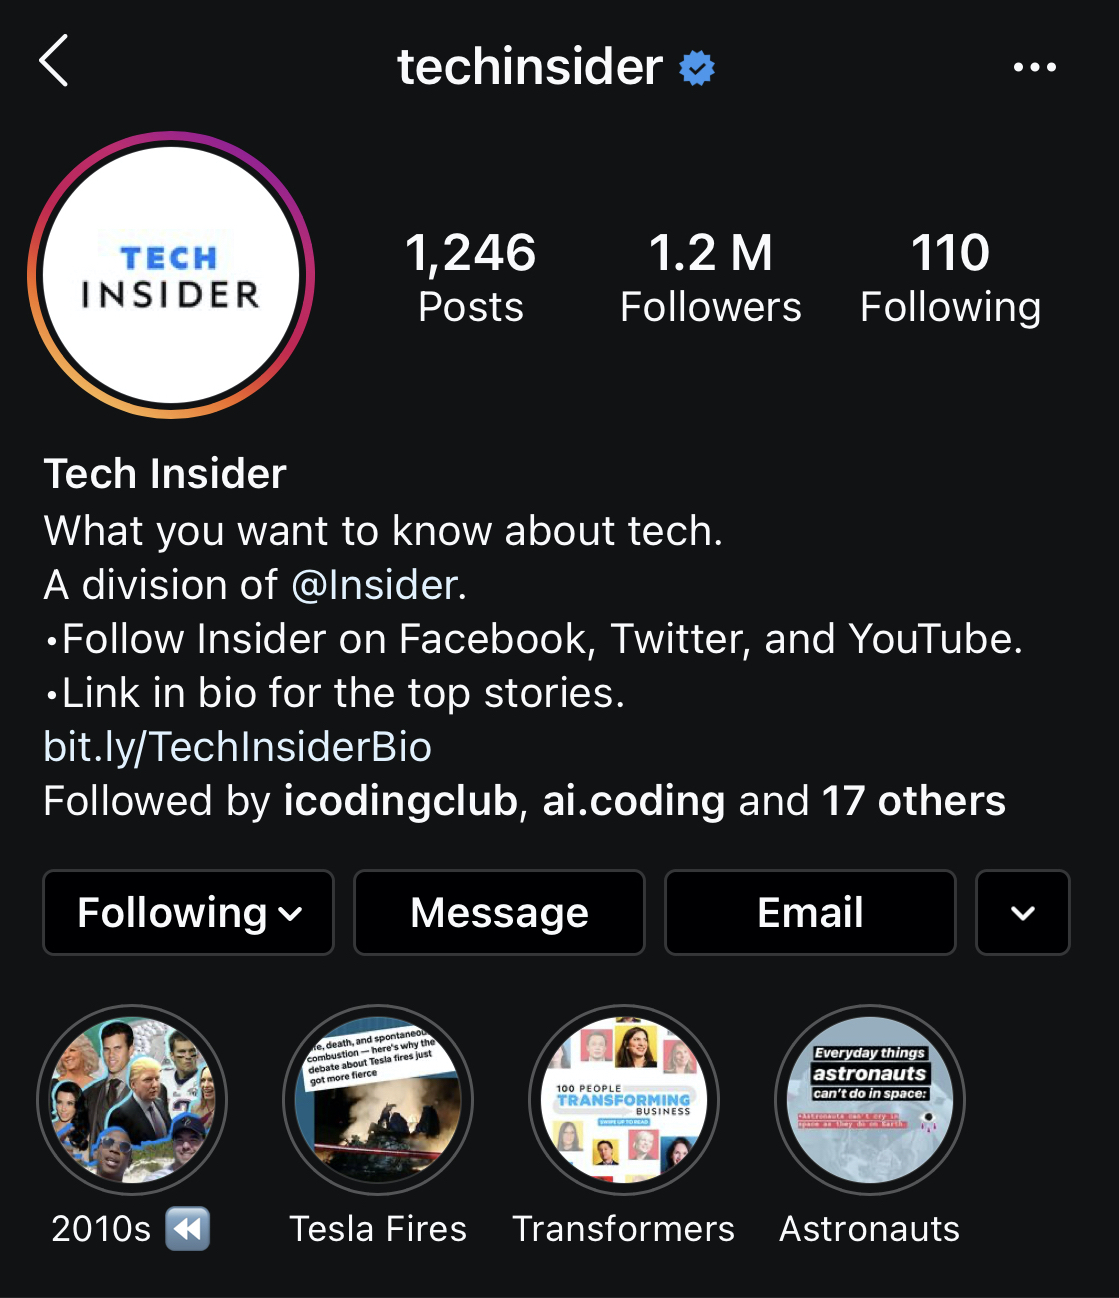
\includegraphics[width=7cm]{instagram_example.jpeg}
%		\end{center}
%	\end{figure}

\begin{figure}
	\begin{center}
		
\includegraphics[width=7cm]{instagram_example2.jpeg}
		\caption{An Instragram user profile overview. This is @bigdataqueen public profile overview.}
		\label{fig:instagram_overview}
	\end{center}
\end{figure}

	The tool that we are critiquing will be the user bio and profile metrics (see figure: \ref{fig:instagram_overview}) from Instagram. The figure shows a cropped image of just the main area that we will be critiquing, that includes all the users' metrics, profile overview and bio. What appears below this section is the users posted photos. As we can see, the user's username is big and bold at the top, with their profile picture just below on the left-hand side. Only to the right of the image is the user's metrics that include how many photos they have posted, how many followers they have and then how many people they are following. These metrics are also displayed in a bold text, bringing the profile viewer's attention immediately onto it. Just below the profile's image and metrics is the user's bio. The user's biography is an area for the user to give the profile viewer some insight into the person behind the profile. This area is smaller in the size of the text and does not have any bold text either. The section below the profile's bio is a little bit of insight to potential other followers you know who follow this profile as if trying to influence to follow this person like other people you follow do, so you should too. While this text is small in size, it has a bold font, so again drawing the views eye away from the bio and more on the influencing metrics. Just below this information is then an area where the profile creator has saved some of the stories that they have created. This area allows the user to view the user's stories whenever they desire, rather than the usual 24-hour window.
	
	While Instagram aims to make connections and to share images across the internet, another focus is also to make sure people are following as many people as possible and viewing as much content as possible. This influencing nature has created a culture of the influencers, who are usually people who have a large following that they receive money or offers for promoting or advertising some form of a product. Millions of consumers trust these influencers. It turns out 86\% of them used influencer marketing since last year, and budgets for influencer marketing are skyrocketing, and 70\% of teens trust influencers more than traditional celebrities \cite{influencers}.  While also, 86\% of women use social media for purchasing advice \cite{influencers}. So as we can see that it is typical for these accounts to have a high number of pictures uploaded and a very high number of followers. This high volume is followers is what gets usually used to perceive someone as an influencer, due to them having a large following to influence.
	
	At the same time, while the user profile's bio does have a more significant space than anything above it. It, however, does not draw the profile viewers eye's attention to it, unlike the profile's metrics, which can get perceived as there getting more of a focus on the creator's metrics and how popular they are, instead of the focus on the creator as an individual. So as women are usually more influenced over social media and them getting judged on how good their metrics are, rather than who they are and what they have created. There is no wonder that social media and Instagram can affect these people's mental health and result in having higher depressive symptom scores, as its not about you as a person but your popularity on a digital platform.

\section{Designed Innovation}

\begin{figure}
	\begin{center}
		
\includegraphics[width=7cm]{instagram_example2.jpg}
		\caption{A design concept of @bigdataqueen new public profile overview.}
		\label{fig:instagram_new_overview}
	\end{center}
\end{figure}

	A design innovation that we have created is to take this profile overview and change the focus (see figure: \ref{fig:instagram_new_overview}). We believe that the profile picture and, most importantly, the creator's bio should be the focus. The focus should be on the person behind the images and content, rather than on the metrics they have. The metrics, should be made less of a priority or even, we believe, be hidden behind a drop-down menu. As if an influences content quality is good, then their metrics, in our opinion, shouldn't matter. Therefore, creating less stress and anxiety about the person's metrics, leading to a worse state of mental health, and promoting the creator behind the content and who they are.


% BALANCE COLUMNS
\balance{}

% REFERENCES FORMAT
% References must be the same font size as other body text.
\bibliographystyle{SIGCHI-Reference-Format}
\bibliography{sample}

\end{document}

%%% Local Variables:
%%% mode: latex
%%% TeX-master: t
%%% End:
